\documentclass[a4paper, 11pt]{article}
\usepackage{graphicx}
\graphicspath{ {./images/} }
\usepackage[utf8]{vietnam}
\usepackage[unicode]{hyperref}
\hypersetup{
    colorlinks=true,
    linkcolor=blue,
    filecolor=magenta,      
    urlcolor=cyan,
}

\usepackage{xcolor}
\usepackage{listings}
\lstset{basicstyle=\ttfamily\small,
  showstringspaces=false,
  commentstyle=\color{red},
  keywordstyle=\color{blue}
}

\usepackage{lmodern}
\usepackage[parfill]{parskip}

\renewcommand{\thefigure}{\arabic{section}.\arabic{figure}}

\renewcommand{\figurename}{Hình}

\renewcommand{\familydefault}{\sfdefault}

% define the title
\author{Nguyen The Minh}
\title{Hiểu về Git}
\begin{document}
% generates the title
\maketitle
\tableofcontents
\newpage

\section{Quản lý version với Git} \label{introduction}

\begin{figure}
\centering
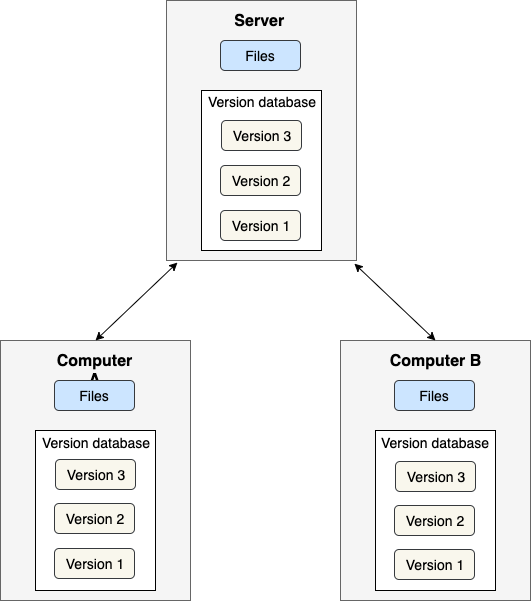
\includegraphics[scale=0.6]{git-overview.png}
\caption{Git là một distributed VCS. Git sử dụng một database để lưu thông tin thay đổi của các files và các version}
\label{fig:git-overview}
\end{figure}

\textbf{Git} là một \textbf{Version Control System - VCS} - hệ thống ghi lại những thay đổi của một tập các files qua thời gian mà sau đó bạn có thể chuyển về một version bất kỳ. Files được quản lý version thường là source code. Git cũng đồng thời là một hệ quản lý version phân tán - Distributed VCS. Điều này có nghĩa là bạn có thể dùng Git để quản lý version cho files trên máy mình - local version control và vừa có thể chia sẻ các version cho người khác, Git sẽ giúp bạn đẩy các thay đổi hay các version lên các server và từ đó bất kỳ ai có quyền có thể lấy các version được chia sẻ về máy cá nhân. Hình~\ref{fig:git-overview} mô tả bức tranh tổng quan của một project được quản lý version bằng Git, trong đó Git sử dụng một database để lưu lại các version của files cũng như tất cả các thông tin cần thiết trong quá trình hoạt động.

Để bắt đầu quản lý version với Git, chúng ta cần tạo một Git \textbf{repository}. Để khởi tạo một repository mới, chúng ta dùng command \footnote{Bài viết sẽ sử dụng command để thao tác với Git, bạn có thể dùng các tool khác có tích hợp Git với ý nghĩa tương tự.} \texttt{git init}. Hay copy một repository có sẵn ở đâu đó (giống như copy thư mục và files). Git cung cấp command \texttt{git clone} để copy một repository từ server về máy cá nhân.

Command bên dưới sẽ tạo một repository mới trong một thư mục mới là git-demo.

\begin{lstlisting}[language=bash]
// Create an empty Git repository
$ git init git-demo
Initialized empty Git repository in git-demo/.git/
\end{lstlisting}

\noindent Để copy một repository có sẵn trên server về máy, sử dụng \texttt{git clone}.

\begin{lstlisting}[language=bash]
// Clone a repository into a new directory
$ git clone git@bitbucket.org:minh/git-demo.git
\end{lstlisting}

Từ trạng thái ban đầu gọi là trạng thái empty, bạn có thể thêm một hay nhiều file vào repository để tạo ra version đầu tiên cho repository. Sau đó chúng ta có thể thêm, sửa, hay xoá các file và tạo ra version mới cho repository. Bạn có thể thấy trong thư mục của một repository sẽ có một thư mục đặc biệt là \textbf{.git}, là nơi được Git sử dụng để lưu các version và tất cả các thông tin khác cần thiết trong quá trình quản lý repository. Thư mục này được coi như một simple database của repository và thông thường thì chúng ta sẽ không trực tiếp động tới thư mục này. Phần còn lại (trừ thư mục \textbf{.git}) được gọi là \textbf{working area} hay \textbf{working tree}, là nơi chúng ta sẽ thao tác trực tiếp như thêm file, sửa file hay xoá file. Hình~\ref{fig:repository-directory-structure} mô tả cấu trúc thư mục của một repository.

\begin{figure}
\centering
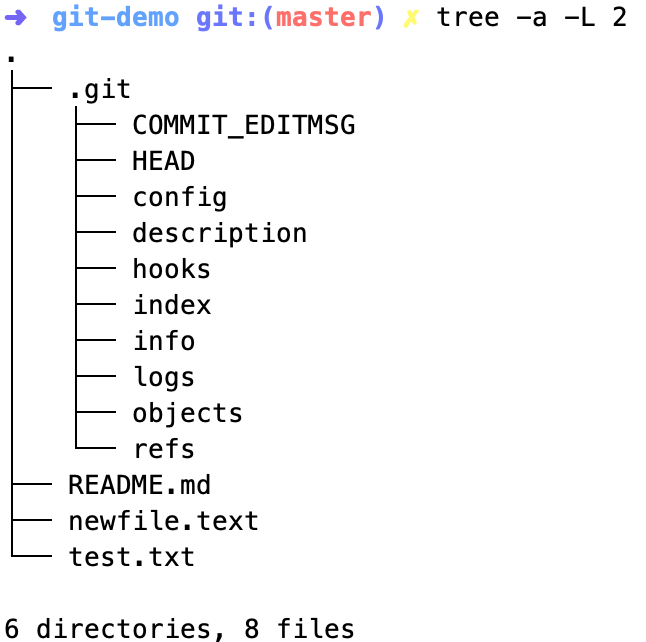
\includegraphics[scale=0.5]{repository-directory.png}
\caption{Cấu trúc thư mục của một repository}
\label{fig:repository-directory-structure}
\end{figure}

Tiếp theo, chúng ta sẽ dùng Git để tạo version mới cho repository của mình và khảo sát xem Git làm nó như thế nào. Chúng ta sẽ bắt đầu từ khi repository là empty, và bạn tạo một file mới trong thư mục của repository (cụ thể là trong \textbf{working tree}).

\begin{lstlisting}[language=bash]
$ echo "Version 1" > test.txt
\end{lstlisting}

Tiếp theo đó là thêm file vào database của repository bằng command \texttt{git add}. Khi này file được gọi là đã \textbf{tracked}, còn trước đó khi chưa được thêm vào repository thì trạng thái của file là \textbf{untracked}. Command \texttt{git add} sẽ tạo ra một version của file và đưa vào một khu vực gọi là \textbf{staging area}.

\begin{lstlisting}[language=bash]
$ git add test.txt
\end{lstlisting}

Bạn có thể dùng command \texttt{git add} để thêm nhiều files vào khu vực \textbf{staging area}. Đến khi bạn quyết định tạo một version mới cho repository thì khi này bạn sẽ sử dụng command \texttt{git commit} để tạo ra một version mới của repository từ \textbf{staging area} hay còn gọi là một \textbf{commit} mới.

\begin{lstlisting}[language=bash]
$ git commit -m "The first commit"
\end{lstlisting}

Như vậy, một version của repository hay còn gọi là một \textbf{commit} sẽ là một tập các version của các files \footnote{Trên thực tế, Git sẽ lưu mỗi version của một file dưới dạng một \textbf{blob} object và lưu một \textbf{tree} object chứa thông tin các files trong cùng một thư mục. Một commit sẽ trỏ tới một tree object.} hay là một \textbf{snapshot}. Hình~\ref{fig:snapshot-stream} mô tả chuỗi các version của một repository giống như một stream of snapshots. Hành động chuyển từ version này sang version khác gọi là \textbf{checkout}. Bạn có thể sử dụng command \texttt{git checkout <commit-id>} để đưa \textbf{working tree} về một version nhất định.

 \begin{lstlisting}[language=bash]
$ git checkout 712838d
\end{lstlisting}

\begin{figure}
\centering
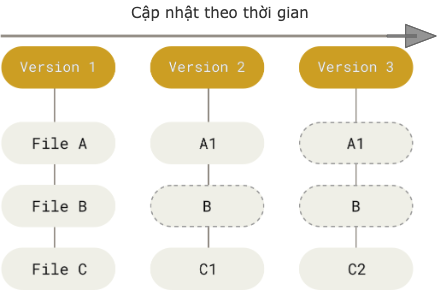
\includegraphics[scale=0.5]{git-snapshot-stream.png}
\caption{Các version của một repository có thể coi như là một series of snapshot theo thời gian}
\label{fig:snapshot-stream}
\end{figure}

Chúng ta sẽ tiếp tục bằng việc tìm hiểu về các trạng thái của một file trong một repository. Hình~\ref{fig:file-status-lifecycle} thể hiện các trạng thái và sự chuyển đổi trạng thái của một file. Trạng thái \textbf{untracked} là khi file chưa được thêm vào repository hay bị xoá khỏi repository. Trạng thái \textbf{staged} là khi file được thêm vào \textbf{staging area} (bằng \texttt{git add}) để tạo version mới từ trạng thái \textbf{untracked} hay \textbf{modified} - file đã thay đổi so với version hiện tại. Từ trạng thái \textbf{staged} chuyển sang \textbf{committed} (bằng \texttt{git commit}) nghĩa là version mới của file được đưa vào một commit mới.

\begin{figure}
\centering
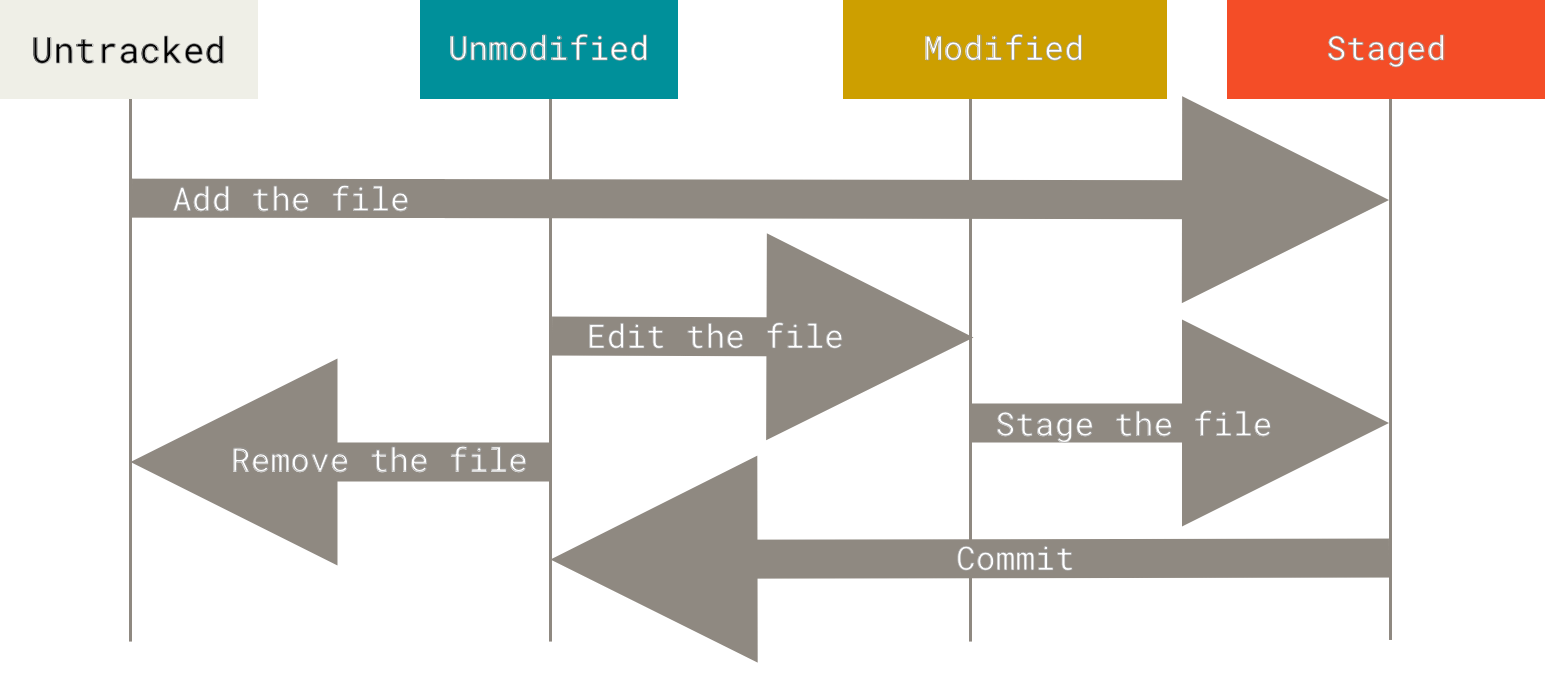
\includegraphics[width=12cm]{lifecycle.png}
\caption{Vòng đời các trạng thái của file}
\label{fig:file-status-lifecycle}
\end{figure}

\clearpage
\section{Git Branching}
\subsection{Git branch là gì?}
Git đưa ra khái niệm \textbf{branch} hay \textbf{nhánh} để chỉ một hướng đi nhất định trong repository. Các hướng đi hay branch là độc lập, do đó chúng ta có thể phát triển song song các chức năng hay các thử nghiệm trên một repository. Hãy xem xét một quy trình phát triển dự án khá thông dụng như sau. Ban đầu dự án có một bộ source code chính và từ đó chúng ta tách ra các hướng khác nhau để phát triển song song. Khi một hướng nào đó kết thúc phát triển thì source code sẽ được gộp (gọi là \textbf{merge}) vào bộ source code chính. Git branch giúp chúng ta thực hiện được mô hình phát triển như vậy, trong đó có một branch chứa bộ source code chính gọi là \textbf{main branch}. Khi cần phát triển song song các tính năng, chúng ta sẽ tách từ main branch ra các nhánh khác gọi là \textbf{feature branch}. Các feature branch sẽ được merge vào main branch sau khi chúng được hoàn thành. 

\begin{figure}
\centering
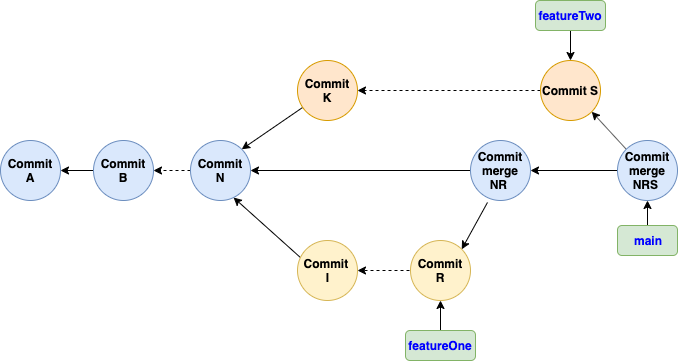
\includegraphics[width=12cm]{git-branch.png}
\caption{Branch và lịch sử commit}
\label{fig:git-branch}
\end{figure}

Hình~\ref{fig:git-branch} mô tả Git branch hoạt động như thế nào. Main branch đang dừng ở \textit{commit N} và từ đó ta tách ra hai branch khác nhau. Sau một thời gian phát triển, branch thứ nhất hoàn thành, dừng ở \textit{commit R}, được merge vào main branch tạo ra một commit mới \textit{commit merge NR}. Khi nhánh thứ hai kết thúc, dừng ở \textit{commit S}, cũng được merge vào main branch tao ra một \textit{commit merge NRS}. Main branch sẽ có lịch sử commit (\textbf{commit history}) như sau:

\texttt{A -> B -> ... -> N -> NR -> NRS}

\noindent Branch thứ nhất sẽ có lịch sử: \texttt{A -> B -> ... -> N -> I -> R}. Còn branch thứ hai sẽ có lịch sử commit là:  \texttt{A -> B -> ... -> N -> K -> S}. Commit phía trước gọi là \textbf{parent} commit. Mỗi commit sẽ có một \textbf{parent} commit, hay không có \textbf{parent} đối với commit đầu tiên, hay là có nhiều \textbf{parent} đối với \textbf{commit merge}. Đối với mỗi branch, Git sẽ lưu một \textbf{reference} để trỏ tới commit cuối cùng của nhánh \textbf{last commit}. Như trong ví dụ ở hình vẽ, Git sử dụng ba reference là \textit{main}, \textit{featureOne}, và \textit{featureTwo} để trỏ tới các \textbf{last commit} của ba nhánh (còn gọi là tracking the last commit của branch). Thêm nữa, Git có một reference trỏ tới branch hiện tại gọi là \textbf{HEAD}. Khi đang ở một branch và bạn tạo ra một commit mới (\texttt{git commit}), Git sẽ tự động dịch chuyển branch reference trỏ tới commit mới. Cũng do đó branch reference còn được gọi là \textbf{movable reference}.

\begin{figure}
\centering
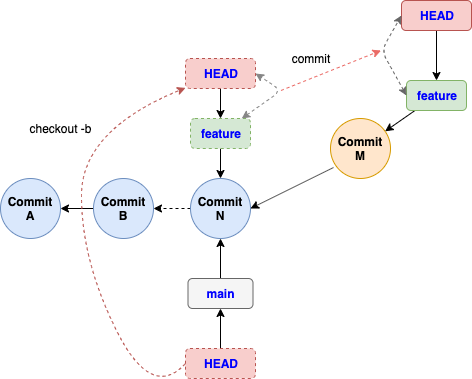
\includegraphics[scale=0.6]{git-reference-move.png}
\caption{Sự di chuyển của \textbf{HEAD} và branch reference}
\label{fig:reference-movation}
\end{figure}

Để tạo một nhánh mới từ một nhánh ban đầu, chúng ta sử dụng command sau.

 \begin{lstlisting}[language=bash]
 // Create and switch to a new branch from the current
$ git checkout -b feature
\end{lstlisting}

Ban đầu chúng ta đang ở main branch, command trên sẽ tạo một branch mới tên là \textit{feature} từ main branch. Git làm điều này bằng cách tạo một \textbf{reference} mới trỏ tới commit mà main branch đang trỏ (last commit của main branch) và đồng thời chuyển \textbf{HEAD} trỏ tới reference mới (feature) này. Như vậy branch hiện tại của chúng ta sẽ là \textit{feature branch}. Khi bạn tạo một commit mới trên feature branch, Git sẽ tự động dịch chuyển \textit{feature branch reference} tới commit mới vừa tạo. Hình~\ref{fig:reference-movation} thể hiện một ví dụ trong quá trình di chuyển của HEAD và branch.

\subsection{Branch merging} \label{merging}
Như đã đề cập ở trên, khi kết thúc phát triển một branch, chúng ta sẽ gộp nó vào main branch. Hành động gộp này gọi là \textbf{merge} branch. \footnote{Trên thực tế, việc merge branch chính là merge các commit lại và tạo ra commit merge. Bạn có thể merge hai hay nhiều commit với nhau.}  Cách git merge branch được mô tả trong hình~\ref{fig:three-way-merge}. Git sử dụng phương pháp \textbf{three-way merging}, trong đó không chỉ hai commit merge với nhau được so sánh và còn so sánh chúng với commit \textbf{common ancestor}, để tạo ra commit merge. Common ancestor của hai commit là commit chung (tổ tiên) mà từ đó hai commit được phát triển lên. Kết quả merge branch được thể hiện trong hình~\ref{fig:merge-result}.

\begin{figure}
\centering
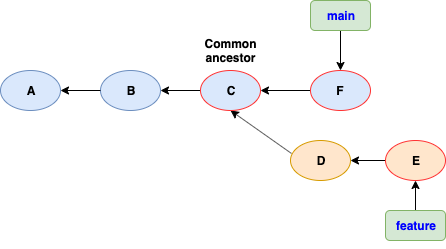
\includegraphics[scale=0.6]{git-three-way-merge.png}
\caption{Git sử dụng phương pháp merge gọi là \textbf{three-way merging}}
\label{fig:three-way-merge}
\end{figure}

\begin{figure}
\centering
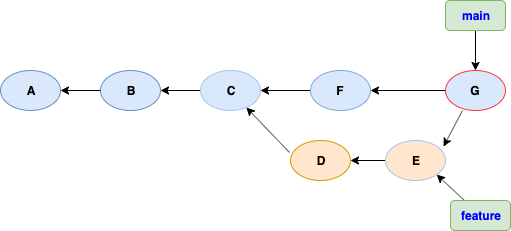
\includegraphics[scale=0.6]{git-merge-result.png}
\caption{Kết quả merge branch, main branch sẽ trỏ tới commit merge}
\label{fig:merge-result}
\end{figure}

Nếu từ khi feature branch được tách ra từ main branch đến khi merge vào main branch mà trên main branch không có thêm commit nào, thì khi đó Git thực hiện \textbf{fast-forward} merge. Fast-forward merge nghĩa là Git không tạo thêm commit (không có thêm commit merge) mà đơn giản là di chuyển main branch reference trỏ tới last commit của feature branch. Hình~\ref{fig:fast-forward-merge} mô tả fast-forward merge của Git.

\begin{figure}
\centering
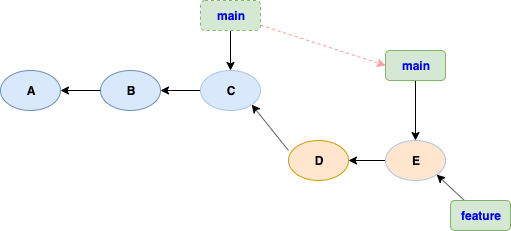
\includegraphics[scale=0.6]{git-fast-forward-merge.png}
\caption{Fast-forward merge}
\label{fig:fast-forward-merge}
\end{figure}

Quá trình merge không phải lúc nào cũng suôn sẻ. Nếu bạn thay đổi cùng một phần của một file trên hai branch đang dùng để merge thì CONFLICT sẽ xảy ra .
\begin{lstlisting}[language=bash]
$ git merge feature
Auto-merging index.html
CONFLICT (content): Merge conflict in index.html 
Automatic merge failed; 
fix conflicts and then commit the result
\end{lstlisting}

Khi có conflict, Git sẽ sử dụng \textbf{conflict maker} ( $<<<<<<$ ) để đánh dấu conflict trong các file. Bạn có thể dùng \texttt{git diff} để xác định các phần maker này và sửa chúng để xử lý CONFLICT (resolve conflicts). 

\begin{lstlisting}[language=html]
<<<<<<< HEAD:index.html
<div id="footer">contact</div>
=======
<div id="footer">
please contact us at support@example.com
</div>
>>>>>>> feature:index.html
\end{lstlisting}

Với những file đã được sửa, bạn cần chỉ cho Git  rằng conflict được được xử lý bằng cách dùng.

\begin{lstlisting}[language=bash]
$ git add <filename>
\end{lstlisting}

\subsection{Remote branches}
Như trong phần \ref{introduction} đã giới thiệu, chúng ta có thể chia sẻ và đồng bộ repository của mình lên nhiều server khách nhau. Git cho phép chúng ta làm điều này bằng việc thêm \textbf{remote repository} (còn gọi là \textbf{upstream repository}) thông qua command \texttt{git remote add <remote-name> <remote-url>}. Còn khi sử dụng \texttt{git clone <remote-url>} thì Git tự động thêm một remote repository với tên là \textbf{origin} có URL là url được clone.

\begin{lstlisting}[language=bash]
$ git remote add github https://github.com/minh/git-demo
\end{lstlisting}

Để đồng bộ thông tin từ một remote repository về máy mình, chúng ta sử dụng command \texttt{git fetch <remote-name>}. Command này sẽ download objects (blobs, commits, ...) và references (branches, tags) từ remote repository về local, bao gồm \textbf{remote branch references}. Remote branches là các references mô tả trạng thái của branches trên remote repository (cụ thể là đang trỏ đến commit nào). Một remote branch sẽ có dạng \texttt{<remote-name>/<branch-name>}. Để download chỉ một remote branch và các objects liên quan, bạn cần chỉ định tên branch \texttt{git fetch <remote-name> <branch-name>}. Command \texttt{git fetch} sẽ tự động tạo một local branch cùng tên (nếu chưa có) tương ứng với một remote branch. Xét ví dụ dưới đây.

\begin{lstlisting}[language=bash]
$ git fetch origin feature
\end{lstlisting}

Ở local sẽ có một branch với tên \texttt{feature} và Git lưu thêm thông tin branch này \textbf{tracking} remote branch \texttt{origin/feature}\footnote{Thông tin tracking remote branch sẽ được Git lưu trong file .git/config.}. Bạn có thể xem danh sách các branch và thông tin tracking remote branch bằng command \texttt{git branch -vv}.

\begin{lstlisting}[language=bash]
$ git branch -vv
develop   73704af [origin/develop] Feature1
feature1  994f6e9 [origin/feature1] Build feature1
master    43208bb [origin/master] Fix input validation
\end{lstlisting}

Git cung cấp một command khác cũng để đồng bộ thông tin từ remote repository là \texttt{git pull <remote>}. Chỉ khác với \texttt{git fetch} là command này sau khi download remote branch thì sẽ thực hiện \textbf{merge} vào local branch đang tracking remote branch đó. Ngoài ra, bạn có thể tự cấu hình tracking remote branch cho branch hiện tại bằng command:

\begin{lstlisting}[language=bash]
$ git branch -u origin/notifyfix
\end{lstlisting}

\noindent Pushing

\noindent Khi bạn muốn chia sẻ một branch với mọi người, bạn cần \textbf{push} branch lên remote repository mà bạn có quyền. Sử dụng \texttt{git push <remote> <branch>}:

\begin{lstlisting}[language=bash]
$ git push origin feature
\end{lstlisting}

\noindent Thực tế thì command trên tương đương với command sau: 

\texttt{git push origin feature:feature}

\noindent Nghĩa là hãy đồng bộ nhánh feature lên nhánh feature của remote. Và đương nhiên, bạn có thể push một nhánh lên một nhánh khác tên trên remote kiểu như  \texttt{git push origin feature:otherBranch}.

\clearpage
\section{Rebasing}

\begin{figure}
\centering
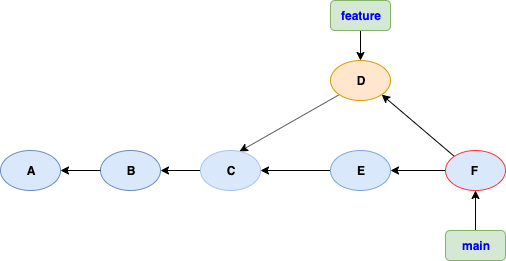
\includegraphics[scale=0.6]{git-merge-commit.png}
\caption{Sử dụng merge để tích hợp nhánh}
\label{fig:merge-integration}
\end{figure}

Như đã thảo luận ở phần \ref{merging}, để tích hợp một nhánh vào nhánh khác (thường là nhánh chính) Git cung cấp công cụ \textbf{merge}. Ngoài ra Git còn cung cấp một công cụ khác là \textbf{rebase} cũng được dùng để tích hợp branch. Chúng ta cùng review lại quá trình merge branch thông qua hình~\ref{fig:merge-integration}. Git thực hiện \textbf{three-way merge} hai commit cuối cùng của hai nhánh (D và E) và commit chung gần nhất (C - the most common ancestor) để tạo ra một commit mới F - gọi là \textbf{commit merge}.

Có một cách khác để tích hợp hai nhánh, đó là áp dụng lại (\textbf{reapply}) thay đổi của commit D lên trên commit C thu được commit mới D' (xem hình~\ref{fig:git-rebase}). Quá trình này gọi là \textbf{rebasing} - reapply commits lên trên một commit khác (base).

\begin{figure}
\centering
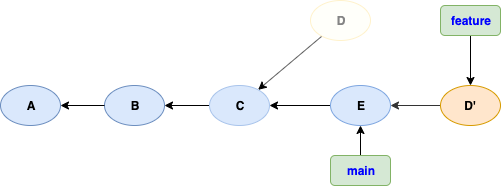
\includegraphics[scale=0.6]{git-rebase.png}
\caption{Rebase commit}
\label{fig:git-rebase}
\end{figure}

\begin{lstlisting}[language=bash]
$ git rebase main //git rebase main feature
$ git checkout main
$ git merge feature
\end{lstlisting}

Sau khi thực hiện rebase, bạn có thể quay lại main branch và thực hiện \textbf{fast-forward merge}. Kết quả như hình~\ref{fig:fast-forward-merge-rebase}. Snapshot (nội dung) của commit D' và commit F ở ví dụ merge là như nhau. Sản phẩm tích hợp cuối cùng là một, tuy nhiên \textbf{rebase} đưa ra một lịch sử commit sáng rõ hơn (clearer commit history) giống như là phát triển tuyến tính (linear history).

\begin{figure}
\centering
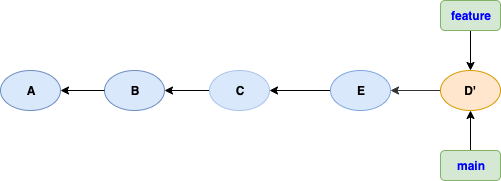
\includegraphics[scale=0.6]{git-merge-rebase.png}
\caption{Rebase commit}
\label{fig:fast-forward-merge-rebase}
\end{figure}

Chúng ta đã minh hoạ cách rebase một commit lên trên môt commit khác. Tiếp theo, chúng ta xét trường hợp rebase nhiều commit lên trên một commit. Giả sử luồng lịch sử như sau và bạn đang ở branch topic.

% Will be printed like 
%         A---B---C topic
%         /
%D---E---F---G master
\begin{verbatim}
      A---B---C topic
     /
D---E---F---G master
\end{verbatim}

\noindent Git sẽ thực hiện \textbf{reapply} lần lượt từng commit trên nhánh topic lên commit cuối của nhánh master. Kết quả rebase nhánh \textit{topic} theo \textit{master} sẽ là:

% Will be printed like 
%				      A'--B'--C' topic
%                       /
%D---E---F---G master
\begin{verbatim}
              A'--B'--C' topic
             /
D---E---F---G master
\end{verbatim}

Quá trình \textbf{reapply} commit lên trên commit base thực ra là một quá trình \textbf{merge} (không phải là three-way) hai commits để tạo ra commit mới rồi xoá commit cũ đi. Việc merge có thể bị \textbf{conflict} (failure), khi đó bạn cần xử lý merge failure và chạy command \textbf{git rebase \texttt{-{}-}continue}. Bạn có thể bỏ qua merge failure bằng \textbf{git rebase \texttt{-{}-}skip} hay huỷ quá trình rebase bằng \textbf{git rebase \texttt{-{}-}abort}.

Một trường hợp khác khi rebase là có một commit nào đó trên topic có nội dung thay đổi giống một commit khác trên nhánh master thì khi đó commit trên topic sẽ được bỏ qua (\textbf{skipped}). Với ví dụ sau, commit A và A' có cùng nội dung thay đổi, commit A sẽ được bỏ qua trong quá trình rebase.
 
% Will be printed like 
%           A---B---C topic
%          /
% D---E---A'---F master
\begin{verbatim}
       A---B---C topic
      /
D---E---A'---F master
\end{verbatim}

\noindent Sau khi rebase, kết quả sẽ là:
% Will be printed like 
%                         B'---C' topic
%                        /
%D---E---A'---F master
\begin{verbatim}
               B'---C' topic
              /
D---E---A'---F master
\end{verbatim}

Rebase là thao tác thay đổi lịch sử commit, các commit được rebase sẽ bị mất đi. Trong trường hợp bạn đã chia sẻ bằng cách \textbf{push} các commit của mình lên server (hay bất kỳ đâu) trước khi thực hiện rebase, nếu ai đó lấy branch của bạn từ server về máy cá nhân thì sau khi họ update lại nhánh này sẽ dẫn đến tình trạng sai lệch. Vì lý do trên, có lẽ là bạn \textbf{không nên rebase các commit đã được chia sẻ}.

\section{Rewriting history - viết lại lịch sử}
Trong quá trình phát triển, bạn có thể muốn thay đổi lại lịch sử của các commit trên local repository của mình. Git cung cấp một số công cụ để giúp bạn thực hiện điều này. Trong phần này, chúng ta sẽ cùng \textit{viết lại lịch sử}.

\subsection{Thay đổi commit cuối cùng} \label{git-amend}
Để thay đổi commit cuối (the last commit) của branch hiện tại, chúng ta sử dụng command \textbf{git commit \texttt{-{}-}amend}. Commit amend sẽ giúp bạn thay đổi \textbf{message} của commit và đồng thời thay đổi nội dụng của commit bằng cách áp dụng các file đã được thêm vào \textbf{staging area} (bằng \texttt{git add} chẳng hạn)\footnote{Trên thực tế, git commit  \texttt{-{}-amend} sẽ tạo một commit mới thay cho commit cũ. Do đó bạn đừng amend commit nào mà mình đã chia sẻ nhé.}. Ví dụ một kịch bản sử dụng commit amend như sau. Sau khi commit, bạn thấy có một lỗi typo (chính tả) trong một file nhưng bạn lại không muốn tạo thêm một commit nữa và lúc này bạn sẽ sử dụng đến commit amend.

\begin{lstlisting}[language=bash]
// Modify the file release.txt, then
$ git add release.txt
$ git commit --amend
// Change commit message or not
\end{lstlisting}

\subsection{Rebase interactive - sửa nhiều commit một lúc}
Git cung cấp một công cụ là \textbf{git rebase \texttt{-{}-}interactive} cho phép bạn sửa một danh sách các commit,  bạn có thể reorder (đổi thứ tự) các commit, hay bạn có thể xoá chúng trong khi rebasing. Đầu tiên, bạn cần xác định commit gọi là \textbf{commit gốc} mà từ đó Git sẽ lấy ra tất cả các commit đằng sau commit này trong nhánh hiện tại để chỉnh sửa.

\texttt{git rebase -i <after-this-commit>}

\noindent Editor của Git sẽ hiện ra danh sách commit đứng sau\footnote{Mặc định là Git sẽ bỏ qua - ignore merge commits. Để rebase merge commits, bạn cần thêm option \texttt{-{}-rebase-merges}.} commit được chọn trong nhánh hiện tại để bạn thực hiện chỉnh sửa. Nội dung của editor nhìn giống (more or less) như sau:

\begin{verbatim}
pick 2d3db49 The oneline of commit after this commit
pick abcdca0 The oneline of the next commit
...
\end{verbatim}

\noindent Trong đó mỗi dòng có cấu trúc là:

 \texttt{<action> <commit-id> <commit-message>}
 
\noindent Các dòng được sắp xếp theo thứ tự commit đằng trước thì sẽ ở dòng trên (thứ tự này ngược với \textit{git log}. Dòng đầu tiên là là commit ngay sau commit đã được chọn làm gốc (this commit). Để reoder các commit thì bạn thực hiện reorder các dòng trên. Để xoá commit thì chúng ta thay \textit{pick} bằng \textit{drop} hay xoá luôn dòng ứng với commit đó đi.
  
Bằng cách thay từ khoá \textit{pick} bằng \textit{edit}, bạn nói với \texttt{git rebase} là sau khi áp dụng (applying) commit đó, hãy dừng lại để bạn có thể chỉnh sửa files và hoặc commit message, amend commit, và tiếp tục rebasing.

Nếu bạn muốn gộp (fold) hai hay nhiều commits lại thành một, hãy thay \textit{pick} bằng \textit{squash} hoặc \textit{fixup} cho commit thứ hai và các commit kế tiếp. Commit gộp sẽ có author của commit đầu tiên. Git cũng đề xuất (suggest) message cho commit gộp bằng cách nối các message của các commit lại với message của commit đầu tiên nếu dùng \textit{squash} hay bỏ qua commit messages khi dùng  \textit{fixup}. 

Để dễ hình dung, chúng ta cùng thử đi qua các ví dụ thường được dùng với \texttt{rebase interactive}.

\textit{}

\textbf{SỬA COMMIT}

Giả sử chúng ta có lịch sử commit như sau:

\begin{verbatim}
a4583ef (HEAD -> master) The fourth commit
1cc1daf The third commit
cd4f3b4 The second commit
e1561d3 The first commit
\end{verbatim}

Và bạn muốn sửa một file trong commit thứ hai. Để làm điều này bạn sẽ rebase interactive trên commit thứ nhất.

\texttt{git rebase -i HEAD\string~3}\footnote{A\string~ hay A\string^ nghĩa là parent commit của A, HEAD\string~3 nghĩa là parent của parent của parent của A, nhưng HEAD\string^3 là parent commit thứ 3 của A.}

Editor sẽ hiện ra nội dung giống như sau:

\begin{verbatim}
pick cd4f3b4 The second commit
pick 1cc1daf The third commit
pick a4583ef The fourth commit

# Rebase e1561d3..a4583ef onto e1561d3 (3 commands)
#
# Commands:
# p, pick <commit> = use commit
# r, reword <commit> = use commit, but edit the commit message
# e, edit <commit> = use commit, but stop for amending
# s, squash <commit> = use commit, but meld into 
#      previous commit
# f, fixup <commit> = like "squash", but discard this commit's 
#      log message
# d, drop <commit> = remove commit
...
\end{verbatim}

Chúng ta sẽ thay keyword \textit{pick} của dòng đầu tiên (commi thứ 2) thành \textit{edit}, sau đó lưu lại.

 \begin{verbatim}
edit cd4f3b4 The second commit
pick 1cc1daf The third commit
pick a4583ef The fourth commit

# Rebase e1561d3..a4583ef onto e1561d3 (3 commands)
...
\end{verbatim}

Quá trình rebase diễn ra và Git sẽ dừng lại ở commit thứ 2 để bạn có thể chỉnh sửa. 

\begin{verbatim}
Stopped at cd4f3b4...  The second commit
You can amend the commit now, with

  git commit --amend

Once you are satisfied with your changes, run

  git rebase --continue
...
\end{verbatim}

Chúng ta sửa file test.txt và sau đó đánh dấu là đã sửa xong (git add), sau đó thực hiện amend, rồi cuối cùng là git rebase \texttt{-{}-}continue.

\begin{lstlisting}[language=bash]
$ echo "Version 2 test fixed" test.txt
$ git add test.txt
$ git commit --amend
$ git rebase --continue
\end{lstlisting}

\textit{}

\textbf{XOÁ COMMIT}

Có với lịch sử ban đầu như ví dụ trước, chúng ta sẽ đổi message của commit thứ hai và xoá commit thứ ba.

\texttt{git rebase -i HEAD\string~3}

Editor sẽ hiện ra nội dung giống như ví dụ trước:

\begin{verbatim}
pick cd4f3b4 The second commit
pick 1cc1daf The third commit
pick a4583ef The fourth commit

# Rebase e1561d3..a4583ef onto e1561d3 (3 commands)
...
\end{verbatim}

Chúng ta sẽ sửa thành như sau và lưu lại.

\begin{verbatim}
pick cd4f3b4 The second commit fixed message
drop 1cc1daf The third commit
pick a4583ef The fourth commit

# Rebase e1561d3..a4583ef onto e1561d3 (3 commands)
...
\end{verbatim}

Việc rebase có thể xảy ra CONFLICT, trong ví dụ này chúng ta xoá commit thứ 3, nhưng có một file trong commit thứ 3 được đưa vào commit thứ 4.

\begin{verbatim}
CONFLICT (modify/delete): other.txt deleted in HEAD and 
modified in a4583ef... The fourth commit. Version a4583ef... 
The fourth commit of other.txt left in tree.
error: could not apply a4583ef... The fourth commit
Resolve all conflicts manually, mark them as resolved with
"git add/rm <conflicted_files>", then run 
"git rebase --continue".
You can instead skip this commit: run "git rebase --skip".
To abort and get back to the state before "git rebase", 
run "git rebase --abort".
Could not apply a4583ef... The fourth commit
\end{verbatim}

Ta sẽ giữ lại file bị CONFLICT ở commit thứ 4 bằng cách sử dụng \texttt{git add}, sau đó chạy command \texttt{git rebase \texttt{-{}-}continue}.

\begin{lstlisting}[language=bash]
$ git add other.txt
$ git rebase --continue
\end{lstlisting}

Editor sẽ hiện ra nội dung để bạn sửa commit message của commit thứ 4. Chúng ta bỏ qua bước này bằng cách giữ nguyên nội dung message. Kết quả thu được như sau (xem bằng \texttt{git log \texttt{-{}-oneline}}):

\begin{verbatim}
8eb2bff (HEAD -> master) The fourth commit
cd4f3b4 The second commit
e1561d3 The first commit
\end{verbatim}

Như bạn thấy sau khi rebase, các commit sẽ được thay thế bằng commit mới có id khác.

\textit{}

\textbf{GỘP COMMIT}

Ví dụ tiếp theo, chúng ta sẽ gộp 3 commits cuối cùng lại với nhau thành một.

\begin{verbatim}
303a838 (HEAD -> master) The fourth commit
37d8ff7 The third commit
95cf866 The second commit
c6c3791 The first commit
\end{verbatim}

Chạy git rebase như sau:

\texttt{git rebase -i HEAD\string~3}

Sau đó thay thế từ khoá \textit{pick} của commit thứ 3 và thứ 4 bằng từ khoá \textit{squash}.

\begin{verbatim}

pick 95cf866 The second commit
squash 37d8ff7 The third commit
squash 303a838 The fourth commit

# Rebase c6c3791..303a838 onto c6c3791 (3 commands)
...
\end{verbatim}

Sau đó Git sẽ suggest message cho commit gộp nhìn như sau:

\begin{verbatim}
# This is a combination of 3 commits.
# This is the 1st commit message:

The second commit

# This is the commit message #2:

The third commit

# This is the commit message #3:

The fourth commit
\end{verbatim}

Bạn có thể sửa message của commit gộp sao cho vừa ý. Ta thu được kết quả được thể hiện qua \texttt{git log} như dưới đây:

\begin{verbatim}
commit 2b9b93d... (HEAD -> master)
Author: Minh <minhnt@nal.vn>
Date:   Wed Feb 3 11:11:00 2021 +0700

    The second commit

    The third commit

    The fourth commit

commit c6c3791...
Author: Minh <minhnt@nal.vn>
Date:   Wed Feb 3 11:06:51 2021 +0700

    The first commit
\end{verbatim}

\textit{}

\textbf{SPLITTING - TÁCH COMMIT}

Trong ví dụ trước, chúng ta thực hiện gộp nhiều commit thành một. Trong ví dụ này, chúng ta sẽ làm điều ngược lại là tách một commit thành nhiều commit. Xét lịch sử commit như sau:

\begin{verbatim}
f9d70b7 (HEAD -> master) The third commit - guideline
1a1dbf7 The second commit - add lib
793c46b The first commit
\end{verbatim}

Chúng ta sẽ tách commit thứ 2 thành hai commit thông qua các bước sau đây.

\textbf{Bước thứ nhất là} bắt đầu interactive rebase với \texttt{git rebase -i <commit>\string^ }, ở đó <commit> là commit bạn muốn tách.

 \texttt{git rebase -i HEAD\string~2} ( = \texttt{git rebase -i 1a1dbf7\string^ } )
 
\textbf{Bước  thứ hai} là đánh dấu commit bạn muốn tách với action \textit{edit}.

\begin{verbatim}
edit 1a1dbf7 The second commit - add lib
pick f9d70b7 The third commit - guideline

# Rebase 793c46b..f9d70b7 onto 793c46b (2 commands)
...
\end{verbatim}

\textbf{Bước tiếp theo}, khi quá trình rebase dừng ở commit thứ 2, thì thực hiện \texttt{git reset HEAD\string^ } để \textit{undo} commit và để các file đã thay đổi ở trạng thái \textit{unstaged}. Khi này bạn có thể thực hiện các thay đổi như mong muốn. Ở đây chúng ta sẽ tạo ra thêm hai commit mới.

\begin{lstlisting}[language=bash]
$ git add math.h // unstaged file
$ git commit -m "Math lib"
$ git add time.h // other unstaged file
$ git commit -m "Time lib"
\end{lstlisting}

\textbf{Cuối cùng}, tiếp tục rebase với \texttt{git rebase \texttt{-{}-}continue}.

Kết quả thu được sẽ là:

\begin{verbatim}
6d94780 (HEAD -> master) The third commit - guideline
62f6a2d Time lib
b349fbf Math lib
793c46b The first commit
\end{verbatim}

\clearpage
\section{Git reset}
\textbf{git-reset} - Đưa HEAD về một trạng thái đặc biệt nào đó.

\textbf{HEAD} là một reference trỏ tới branch hiện tại. Còn branch hiện tại lại trỏ tới commit cuối cùng trên branch đó. Tổng quát mà nói, HEAD sẽ trỏ tới commit cuối cùng trên branch hiện tại hay gọi là \texttt{current branch head}. Và Git cho phép bạn đưa HEAD vì bất kỳ trạng thái nào bằng cách sử dụng \textbf{git reset}.

\textbf{Working directory} là nơi chứa các file ở trạng thái hiện tại của repository. Khi bạn thực hiện chuyển repository sang trạng thái khác (commit hay branch khác), chẳng hạn bằng \texttt{git checkout <commit>}, working directory sẽ chứa tất cả các file của trạng thái đó (\textbf{last checked out}). Bạn có thể thay đổi nội dung các file, thêm hay xoá các file trong working directory trước khi đưa chúng vào \textbf{staging area} và rồi đưa vào lịch sử (commit to history).

\textbf{INDEX - staging area} là nơi Git lưu trữ các file và thông tin sẽ được dùng để tạo commit tiếp theo. Cụ thể là INDEX chứa nội dung tất cả các file ở trạng thái hiện tại (last checked out) và cộng thêm các file bạn đã sửa, xoá hay thêm mới (sử dụng git add, git rm) - các file này được Git tạo version mới. Khi bạn tạo commit mới, \textbf{git commit} sẽ convert INDEX thành tree object cho commit mới này (commit sẽ trỏ tới tree object).

Command sau giúp bạn xem nội dung của INDEX.

\begin{lstlisting}[language=bash]
$ git ls-files -s
100644 9b2567b... 0	README.md
100644 cb45571... 0	guideline.md
100644 86ceb58... 0	math.h
100644 90700e9... 0	time.h
\end{lstlisting}

\begin{figure}
\centering
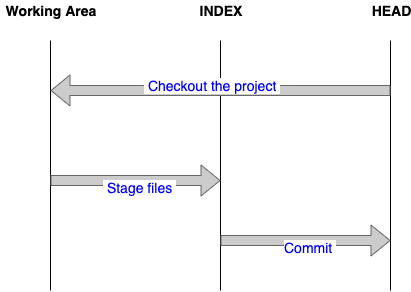
\includegraphics[scale=0.6]{git-workflow.png}
\caption{Git workflow - luồng ghi nhận commit}
\label{fig:git-workflow}
\end{figure}

Bạn có thể hình dung git workflow như hình vẽ~\ref{fig:git-workflow}.

Trong bài viết này, chúng ta sẽ sử dụng git-reset với cấu trúc như sau.

\textbf{git reset [<mode>] [<commit>]}

Cấu trúc này sẽ chuyển (reset) HEAD về <commit> và có thể cập nhật INDEX (reset nó về tree của commit)\footnote{Commit sẽ trỏ tới tree object, tree object sẽ chứa reference trỏ tới các blob objects và có thể chứa subtree khác.} và Working directory tuỳ thuộc theo <mode>. Nếu không cung cấp mode thì mặc định sẽ là \textbf{-{}-mixed}. Chúng ta thường sẽ sử dụng một trong các mode sau:

\textbf{-{}-soft}

Không thay đổi INDEX cũng như working directory (đương nhiên là reset HEAD về <commit> như các mode khác). Kết quả là các file thay đổi sẽ được \textbf{git status} thông báo là "Changes to be committed". Nếu bạn chạy git commit thành một commit mới sẽ được tạo có base (parent) là HEAD đã reset (tất nhiên là HEAD và branch lúc này sẽ trỏ tới commit mới).

\textbf{-{}-mixed}

Reset INDEX nhưng không reset working directory. Nghĩa là các file thay đổi sẽ không được git status thông báo dành cho commit (not marked for commit).

\textbf{-{}-hard}

Reset INDEX và working directory. Mọi thay đổi với các file bắt đầu từ <commit> sẽ bị bỏ qua.

\subsection{Các ví dụ git-reset}

\textbf{Undo add}

\begin{lstlisting}[language=bash]
$ edit
$ git add test.txt
$ git reset HEAD
\end{lstlisting}

\textbf{Undo một commit và redo - làm lại}

\begin{lstlisting}[language=bash]
$ git commit ...
$ git reset --soft HEAD^      (1)
$ edit                        (2)
$ git commit -a -c ORIG_HEAD  (3)
\end{lstlisting}

1. Sau khi commit, bạn cảm thấy chưa ổn và muốn sửa lại nó.

2, 3. Bạn chỉnh sửa sau đó commit lại sửa dụng log message của HEAD cũ.

Như đã trình bày ở mục~\ref{git-amend}, ví dụ này có thể được thực hiện bằng \textbf{git amend} 

\textbf{Undo các commit hoàn toàn}

\begin{lstlisting}[language=bash]
$ git commit ...
$ git reset --hard HEAD~3   (1)
\end{lstlisting}

1. Bạn không muốn thấy ba commit cuối HEAD, HEAD\string^, HEAD\string~2 nữa.

\subsection{Công cụ tương tự reset}
Có một số công cụ gần giống với git-reset đó là:

\begin{figure}
\centering
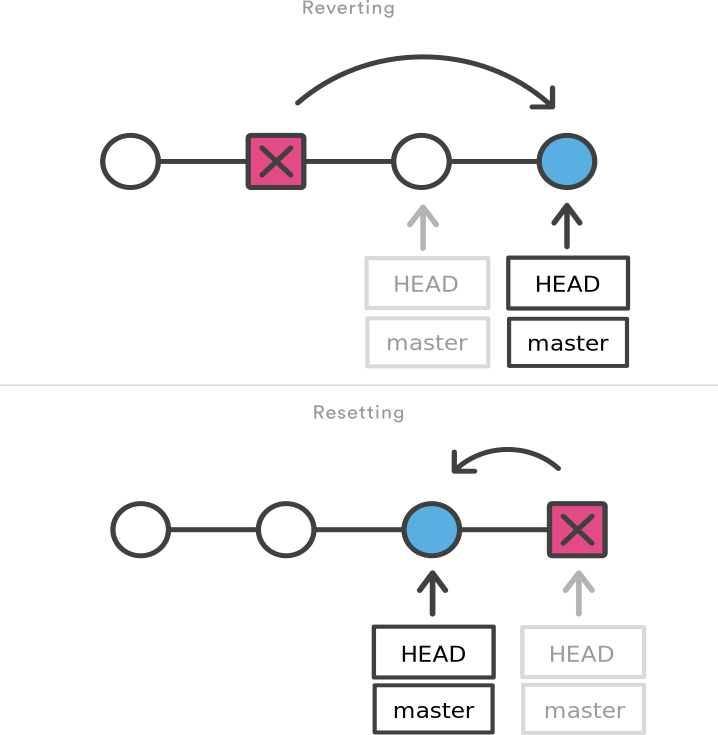
\includegraphics[scale=0.4]{git-revert-vs-reset.png}
\caption{Mô hình hoạt động của git revert và git reset}
\label{fig:git-revert}
\end{figure}

\begin{itemize}
\item \textbf{git revert <commit>} - Chuyển trạng thái của repository về <commit>, có vẻ giống reset nhưng git-revert không làm thay đổi lịch sử (không chuyển HEAD về commit, không thay đổi INDEX) mà tạo commit mới (commit revert) với nội dung giống <commit> chỉ khác parent là commit cuối cùng (cũng là HEAD hiện tại), rồi trỏ HEAD vào commit mới này. Hình~\ref{fig:git-revert} mô tả hoạt động của git-revert. Git revert thường được dùng để undo các thay đổi đã public. Khi đã public thì bạn nên tránh thay đổi lịch sử.
\item \textbf{git restore} - Khôi phục (restore) files trong working directory từ INDEX hay một commit nào đó. Command này không cập nhật branch của bạn. 
\end{itemize}

\section{Tổng kết}
Chúng ta đã đi qua các khái niệm và các chức năng cơ bản cũng như thông dụng của Git. Để hiểu hơn các chức năng khác cũng như hiểu rõ các command của Git, bạn cần tham khảo thêm tài liệu \href{https://git-scm.com/docs}{Git docs}. Và hơn nữa, bạn cần tự mình đặt ra nghi vấn cũng như tự thực hành để thực chứng những gì đọc được. Khi bạn đã hiểu rõ về Git, bạn có thể tự tin sử dụng Git và phát triển dự án của mình. Chúc các bạn sử dụng Git một cách thành thạo và thật là dễ dàng!

\end{document}
